\chapter{Einleitung}
Einleitung
Motivation
Referenz auf führere IDPs (Quellen!)
didaktisches Konzept, kurz
Aufbau der Dokumentation, inkl. Benennung wer hat was gemacht (Benotung)

% Keine Beschreibung der Algorithmen an sich!

\chapter{Aufbau der Webanwendungen}
funktionale Beschreibung der Apps
jedes Tab

\section{Algorithmus von Floyd-Warshall}
Besonderheiten Visualisierung
Forschungsfragen

\section{Algorithmus von Hierholzer (Mark)}
Besonderheiten Visualisierung
Forschungsfragen

\section{Algorithmus von Hopcroft und Karp}
Besonderheiten Visualisierung
Forschungsfragen

\section{Ungarische Methode}
Besonderheiten Visualisierung
Forschungsfragen

\section{Chinese Postman Problem}
Besonderheiten Visualisierung
Forschungsfragen

\chapter{Implementierung}

\section{Installation (Mark)}
Zur Installation sind keine speziellen Anforderungen zu erfüllen. Die Webapplikationen wurden vollständig mittels HTML5, JavaScript und CSS implementiert, sodass keine zusätzliche serverseitige Software benötigt wird. Zum Aufrufen der Anwendungen wird ein moderner Webbrowser benötigt.

Die Bereitstellung erfolgt über den Online Dienst GitHub, der das verteile Versionskontrollsystem Git benutzt. 
Alle Anwendungen liegen in einem gemeinsamen Repository, welches unter \url{https://github.com/herzog31/adv-graph-algorithms} erreichbar ist. Zur Installation kann man entweder auf der Repository Seite die letzte freigegebene Version (Release) als Zip oder Tar Archiv herunterladen oder die aktuellste Version des Repositories mittels folgendem Befehl in das aktuelle Verzeichnis kopieren.

\begin{figure}[h!]
\begin{lstlisting}[language=Bash]
git clone -b master https://github.com/herzog31/adv-graph-algorithms.git
\end{lstlisting}
\caption[Repository Kopieren]{Befehl zum Kopieren des GitHub Repositories}\label{fig:listing-github}
\end{figure}

Um die Anwendungen als Webanwendungen online bereitzustellen wird ein Webserver benötigt. Hier emfiehlt sich die Installation des Apache oder nginx  HTTP Servers.

Die lokale Ausführung ist ohne einen Webserver möglich. Verschiedene Webbrowser besitzen allerdings eine Sicherheitsrichtlinie, die das Öffnen von lokalen Dateien über JavaScript verbieten. Diese Sicherheitsrichtline kann jedoch durch spezielle Einstellungen umgangen werden. Für Google Chrome ist dies über den Start Parameter \texttt{--allow-file-access-from-files} möglich.

\section{MathJAX (Mark)}
Unter den Tabs "Beschreibung des Algorithmus" werden die komplizierte Algorithmen, wie bspw. die Ungarische Methode, in möglichst einfachen Worten als Fließtext erklärt. Wir gehen davon aus, dass der Nutzer während der Bearbeitung der Forschungsaufgaben, verschiedene Sachverhalte in der Algorithmenbeschreibung nachschlagen muss. Das wiederholte Lesen von vollständigen Absätzen wollten wir allerdings vermeiden.

Dazu haben wir zusätzlich zur textuellen Beschreibung, wichtige Punkte der Algorithmen auch als mathematische Formeln dargestellt. Der Nutzer erlangt so durch das erste Lesen der Beschreibung ein Grundverständnis der Algorithmen und kann während der Bearbeitung aufkommende Fragen durch die dargestellten Formeln schneller erschließen.

Zur Darstellung der Formeln in den Webapplikationen verwenden wir JavaScript Bibliothek MathJAX\footnote{https://www.mathjax.org/}. Diese ist frei unter der Apache-Lizenz erhältlich und wird u.a. auch von Wikipedia zur Darstellung jeglicher mathematischer Ausdrücke genutzt. Mit der Bibliothek ist es möglich mit LaTeX beschriebene Ausdrücke als SVG oder PNG im Webbrowser zu rendern. 

Damit die Bibliothek in den Webanwendungen genutzt werden kann, muss sie wie folgt eingebunden werden (vgl. Abbildung~\ref{fig:listing-mathjax-include}.

\begin{figure}[h!]
\begin{lstlisting}[language=HTML]
<script type="text/javascript" src="../library/js/mathjax/MathJax.js?config=TeX-AMS-MML_SVG.js&locale=de"></script>
<script type="text/x-mathjax-config">
	MathJax.Hub.Config({
		showMathMenu: false,
		showMathMenuMSIE: false
	});
</script>
\end{lstlisting}
\caption[MathJAX Einbindung]{Einbinden der MathJAX Bibliothek}\label{fig:listing-mathjax-include}
\end{figure}

Nach der Einbindung werden sämtliche LaTeX Ausdrücke welche sich zwischen den Begrenzungszeichen \texttt{\textbackslash(} und \texttt{\textbackslash)} befinden, automatisch übersetzt. In einem Beispiel wird hier der HTML Code in Abbildung~\ref{fig:listing-mathjax-example-html} von MathJAX im Browser gerendert (vgl. Abbildung~\ref{fig:mathjax-example-img}.

\begin{figure}[h!]
\begin{lstlisting}[language=HTML]
<p style="text-align: center;">
	\(\Delta = \min\limits_{s \in S\ \wedge\ y \in Y \setminus T}\{l(s) + l(y) - w(s,y)\}\)
</p>
\end{lstlisting}
\caption[MathJAX Beispiel]{MathJAX Beispiel: HTML Code}\label{fig:listing-mathjax-example-html}
\end{figure}

\begin{figure}[h!]
	\centering
	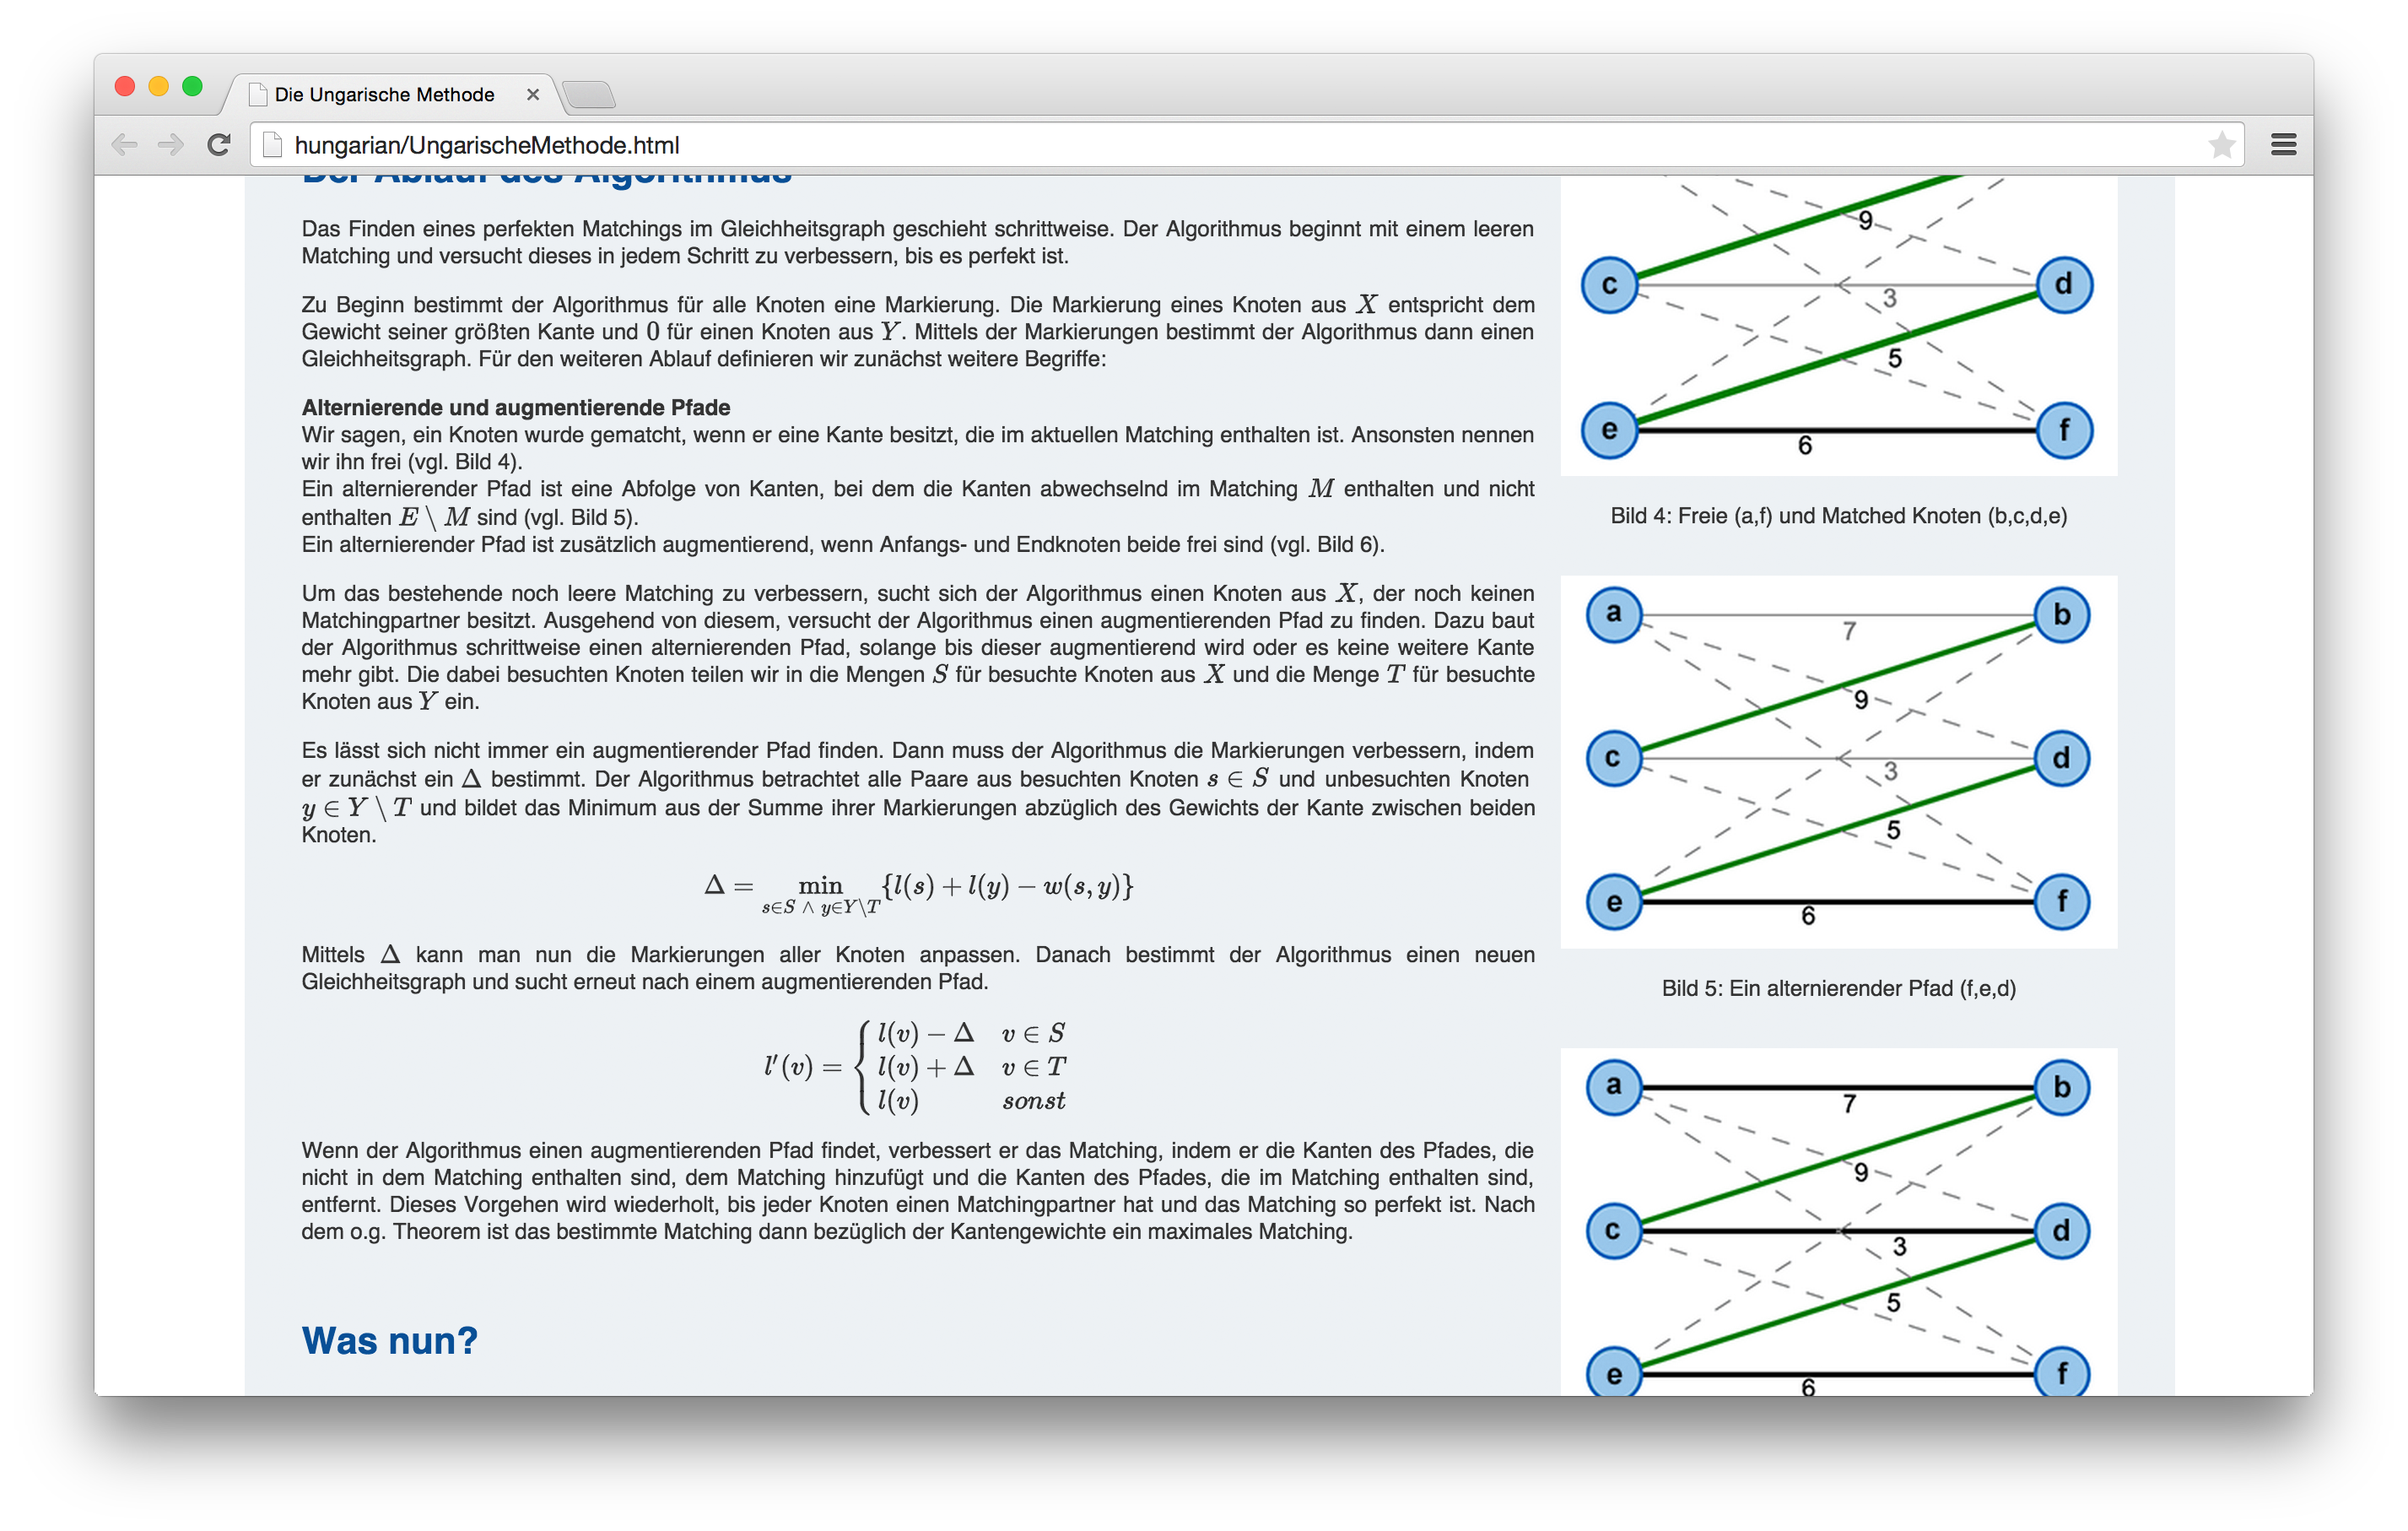
\includegraphics[width=\textwidth]{figures/mathjax-example}
	\caption[MathJAX Beispiel]{MathJAX Beispiel: Darstellung im Browser}\label{fig:mathjax-example-img}
\end{figure}

Werden Ausdrücke zur Laufzeit in das DOM mittels JavaScript eingefügt, so müssen diese separat übersetzt werden (vgl. Abbildung~\ref{fig:listing-mathjax-render}).

\begin{figure}[h!]
\begin{lstlisting}[language=JavaScript]
MathJax.Hub.Queue(["Typeset", MathJax.Hub]);
\end{lstlisting}
\caption[MathJAX Rendern]{Befehl zum erneuten Rendern von Ausdrücken im HTML Dokument}\label{fig:listing-mathjax-render}
\end{figure}

\section{Bipartite Graphen}
Motivation
Beispiel

\section{Multigraphen}
Motivation
Beispiel

\section{Zufällig generierte Fragen (Mark)}
Motivation
Beispiel

\section{Gemeinsam genutzte Dateien (Mark)}
Motivation
Beispiel

\chapter{Zusammenfassung}
Zusammenfassung der wesentlichen Punkte